\documentclass[a4paper]{article}

%·······························································································
%                                _    _                _           
%                               | |  | |              | |          
%                               | |__| | ___  __ _  __| | ___ _ __ 
%                               |  __  |/ _ \/ _` |/ _` |/ _ \ '__|
%                               | |  | |  __/ (_| | (_| |  __/ |   
%                               |_|  |_|\___|\__,_|\__,_|\___|_|   
%·······························································································

% Packages import
\usepackage[spanish]{babel}     % Spanish language support
\usepackage[utf8]{inputenc}     % UTF-8 encoding
\usepackage[T1]{fontenc}        % Proper font encoding
\usepackage{geometry}           % Page layout
\usepackage{titlesec}           % Custom section titles
\usepackage{lmodern}            % Modern font
\usepackage{fancyhdr}           % Header and footer
\usepackage{graphicx}           % Inserting images
\usepackage{anyfontsize}        % Arbitrary font size
\usepackage{listings}           % Code formatting
\usepackage{caption}            % Caption customizing
\usepackage{float}              % Image placing
\usepackage{sourcesanspro}
\usepackage{array}
\usepackage[dvipsnames,x11names,table]{xcolor}
\usepackage[colorlinks=true,linkcolor=black,urlcolor=Emerald]{hyperref}

% Packages configurations {{{

    % Adjust margins
    \geometry{a4paper, margin=2.5cm}

    % Change font family
    \renewcommand{\familydefault}{\sfdefault}
    
    % Change default command to resize all text
    \renewcommand{\normalsize}{\fontsize{13}{16}\selectfont}

    % Change table's cells padding
    \setlength{\tabcolsep}{12pt}
    \renewcommand{\arraystretch}{1.5}
    
    % Header/Footer settings
    \fancyfoot[C]{\thepage}

    % Shell prompt code
    \lstdefinestyle{shellprompt}{
        backgroundcolor=\color{black},
        basicstyle=\fontsize{11}{20}\ttfamily\color{white},
        keywordstyle=\color{NavyBlue},
        commentstyle=\color{white},
        stringstyle=\color{green},
        breaklines=true,
    }

    % Define the style for code with line numbers
    \lstdefinestyle{normalcode}{
        numbers=left,         % Display line numbers on the left
        numberstyle=\tiny,    % Small size for the line numbers
        stepnumber=1,         % Number every line
        numbersep=5pt,        % Space between line numbers and code
        backgroundcolor=\color{lightgray}, % Background color of code block
        basicstyle=\ttfamily\footnotesize, % Set font to typewriter and small size
    }

    % Set default listings style to shellprompt
    \lstset{style=shellprompt}

% }}}

\hyphenpenalty=10000  % Avoid hyphenation
\exhyphenpenalty=10000
\sloppy  % Loosens the strictness of the justification algorithm
\newcommand{\textgap}{\vspace{1em}}

% Metadata {{{

    % Title
    \title{Sistemas Cooperativos y Gestión de Contenidos}
    
    % Author
    \author{Juan Manuel Segura Duarte}

% }}}













%·······························································································
%                     _____                                        _   
%                    |  __ \                                      | |  
%                    | |  | | ___   ___ _   _ _ __ ___   ___ _ __ | |_ 
%                    | |  | |/ _ \ / __| | | | '_ ` _ \ / _ \ '_ \| __|
%                    | |__| | (_) | (__| |_| | | | | | |  __/ | | | |_ 
%                    |_____/ \___/ \___|\__,_|_| |_| |_|\___|_| |_|\__|
%·······························································································
\begin{document}

% Cover Page
\begin{titlepage}
    \centering
    \vspace*{3cm}  % Space at the top
    {\Huge \textbf{SCGC Práctica 2}} % Custom title
    \vspace{1cm}
    
    {\Large Sistemas Cooperativos y Gestión de Contenidos: Desarrollo de la 2ª práctica} % Subtitle
    
    
\includegraphics[width=0.5\textwidth]{images/ugr-logo.png}
    \vspace{1cm}
    
    \textbf{\Large Juan Manuel Segura Duarte} % Author name
\end{titlepage}
\newpage

% Table of Contents page
\thispagestyle{empty}
\tableofcontents

%%%%%%%%%%%%%%%%%%%%%%%%%%%%%%%%%%%%%%%%%%%%%%%%%%%%%%%%%%%%%%%%%%%%%%%%%%%%%%%%%%%%%%%%%%%%%%%%%%
%%%%%%%%%%%%%%%%%%%%%%%%%%%%%%%%%%%%%%%%%%%%%%%%%%%%%%%%%%%%%%%%%%%%%%%%%%%%%%%%%%%%%%%%%%%%%%%%%%
%%%%%%%%%%%%%%%%%%%%%%%%%%%%%%%%%%%%%%%%%%%%%%%%%%%%%%%%%%%%%%%%%%%%%%%%%%%%%%%%%%%%%%%%%%%%%%%%%%

% Start numbering in this page (after the title page and index)
\newpage
\pagenumbering{arabic}
\setcounter{page}{1}

\section{Problema a resolver}

``Carnicería Segura'' (de aquí en adelante \textit{Negocio}) es un negocio familiar que lleva operando durante decadas en un pequeño pueblo granadino, ofreciendo productos tradicionales de alta calidad. Sin embargo, como muchos negocios locales, enfrenta dificultades en su adaptación al entorno digital, lo que limita su alcance y crecimiento.

\textgap

Actualmente, el Negocio no cuenta con una presencia online efectiva, lo que genera varios inconvenientes tanto para la empresa como para sus clientes:

\subsection{Problemas identificados}
\begin{enumerate}

    \item Falta de visibilidad y dependencia del boca a boca
    \begin{itemize}

        \item El Negocio no tiene una página web ni perfiles activos en redes sociales.

        \item Los clientes actuales conocen el Negocio por referencias personales o por haber pasado físicamente frente a la tienda.

        \item Potenciales clientes fuera del pueblo no pueden descubrir el Negocio a través de búsquedas en Internet.

    \end{itemize}


    \item Dificultad para acceder a información clave
    \begin{itemize}

        \item No existe un catálogo digital donde los clientes puedan consultar productos, precios o disponibilidad.

        \item No hay un canal de comunicación directa más allá de llamadas telefónicas o visitas presenciales.

    \end{itemize}


    \item Ausencia de pedidos por encargo en línea
    \begin{itemize}

        \item Actualmente, los pedidos especiales deben realizarse únicamente en persona o por teléfono, lo que resulta poco práctico para muchos clientes.

        \item La falta de un sistema de reservas o pedidos digitales hace que el Negocio dependa de la disponibilidad de los empleados para atender llamadas y tomar notas manualmente.

    \end{itemize}


    \item Poca flexibilidad para promociones y novedades
    \begin{itemize}

        \item No hay un medio para informar sobre descuentos, promociones especiales o nuevos productos de manera efectiva.

        \item El Negocio podría beneficiarse de una sección de noticias donde anunciar cambios de horario, ofertas temporales o introducción de nuevos productos.

    \end{itemize}


    \item Dificultades en la fidelización de clientes
    \begin{itemize}

        \item La falta de una base de datos de clientes dificulta sobremanera realizar estrategias de fidelización, como el envío de boletines informativos o promociones exclusivas.

    \end{itemize}

\end{enumerate}



\subsection{Objetivo del proyecto}

Para resolver estos problemas, se propone el desarrollo de un sistema gestor de contenidos (CMS, por sus siglas en inglés, \textit{Content Management System}) basado en Wordpress que permita al Negocio tener una presencia online funcional y eficiente. La finalidad de este es:

\begin{itemize}

    \item Facilitar la visibilidad del Negocio, permitiendo que clientes potenciales lo encuentren en Internet.
    
    \item Ofrecer un catálogo de productos accesible, con imágenes, descripciones y precios.

    \item Permitir la realización de pedidos por encargo, optimizando la comunicación con los clientes.

\end{itemize}

Crear una sección de noticias y promociones, manteniendo a los clientes informados sobre novedades y ofertas.
Simplificar el contacto con los clientes, integrando formularios de consulta y enlaces a redes sociales.
Garantizar un diseño accesible y \textit{responsive}, para que pueda ser usado cómodamente desde móviles y ordenadores.

\textgap

Con esta solución, el Negocio modernizará su forma de operar sin perder su esencia tradicional, mejorando la experiencia tanto para los dueños del Negocio como para sus clientes.


%%%%%%%%%%%%%%%%%%%%%%%%%%%%%%%%%%%%%%%%%%%%%%%%%%%%%%%%%%%%%%%%%%%%%%%%%%%%%%%%%%%%%%%%%%%%%%%%%%
%%%%%%%%%%%%%%%%%%%%%%%%%%%%%%%%%%%%%%%%%%%%%%%%%%%%%%%%%%%%%%%%%%%%%%%%%%%%%%%%%%%%%%%%%%%%%%%%%%
%%%%%%%%%%%%%%%%%%%%%%%%%%%%%%%%%%%%%%%%%%%%%%%%%%%%%%%%%%%%%%%%%%%%%%%%%%%%%%%%%%%%%%%%%%%%%%%%%%

\section{Datos del cliente}

\begin{table}[ht]
    \centering
    \begin{tabular}{| >{\raggedright\arraybackslash} p{0.2\linewidth} | p{0.7\linewidth} |}
        \hline
        \cellcolor{Snow2} Nombre del comercio & Carnicería Segura \\
        \hline
        \cellcolor{Snow2} Ubicación & Villa de Otura, Granada \\
        \hline
        \cellcolor{Snow2} Tipo de productos & Carnes frescas, embutidos, productos curados y pedidos especiales por encargo. \\
        \hline
        \cellcolor{Snow2} Público objetivo & Habitantes del pueblo y zonas cercanas, así como clientes que buscan productos tradicionales. \\
        \hline
    \end{tabular}
\end{table}


Necesidades identificadas:
\begin{itemize}

    \item Tener una web informativa y fácil de gestionar.

    \item Permitir que los clientes consulten productos disponibles y sus precios.

    \item Ofrecer una sección de noticias/promociones.

\end{itemize}


%%%%%%%%%%%%%%%%%%%%%%%%%%%%%%%%%%%%%%%%%%%%%%%%%%%%%%%%%%%%%%%%%%%%%%%%%%%%%%%%%%%%%%%%%%%%%%%%%%
%%%%%%%%%%%%%%%%%%%%%%%%%%%%%%%%%%%%%%%%%%%%%%%%%%%%%%%%%%%%%%%%%%%%%%%%%%%%%%%%%%%%%%%%%%%%%%%%%%
%%%%%%%%%%%%%%%%%%%%%%%%%%%%%%%%%%%%%%%%%%%%%%%%%%%%%%%%%%%%%%%%%%%%%%%%%%%%%%%%%%%%%%%%%%%%%%%%%%

\section{Proceso de análisis de requisitos}

Para desarrollar el CMS, es necesario definir requisitos clave que permitan cubrir las necesidades del Negocio.

\subsection{Requisitos funcionales}
\begin{itemize}

    \item Página de inicio con fotos de productos destacados y enlaces a secciones clave.

    \item Menú de navegación estructurado con acceso a noticias, productos y contacto.

    \item Sección de noticias para promociones, cambios de horario y novedades.

    \item Catálogo de productos con descripciones, imágenes y precios.

    \item Formulario de contacto para consultas y pedidos por encargo.

    \item Sección de historia del Negocio.

    \item Registro de usuarios, con conteo de pedidos realizados, para fidelización de clientes.

    \item Integración de un widget de productos destacados en la página principal.

\end{itemize}


\subsection{Requisitos técnicos}
\begin{itemize}

    \item Optimización SEO para mejorar el posicionamiento en buscadores.

    \item Seguridad (HTTPS, protección de datos en formularios).

    \item Cumplimiento del RGPD para el manejo de datos de clientes.

    \item Cumplir con las guías del WCAG.

\end{itemize}


%%%%%%%%%%%%%%%%%%%%%%%%%%%%%%%%%%%%%%%%%%%%%%%%%%%%%%%%%%%%%%%%%%%%%%%%%%%%%%%%%%%%%%%%%%%%%%%%%%
%%%%%%%%%%%%%%%%%%%%%%%%%%%%%%%%%%%%%%%%%%%%%%%%%%%%%%%%%%%%%%%%%%%%%%%%%%%%%%%%%%%%%%%%%%%%%%%%%%
%%%%%%%%%%%%%%%%%%%%%%%%%%%%%%%%%%%%%%%%%%%%%%%%%%%%%%%%%%%%%%%%%%%%%%%%%%%%%%%%%%%%%%%%%%%%%%%%%%

\section{Propuesta de diseño}

El diseño del CMS busca ser claro, atractivo y funcional, garantizando una experiencia de usuario sencilla.

\subsection{Comparaciones}

Tras investigar algunas páginas de carnicerías hubo una que resaltó por su diseño elegante y sencillo:
\href{https://carniceriasalbert.com/}{Carnicerías Albert (Alicante)}

\textgap

En la siguiente imagen se puede ver la \textit{Landing page} con el menú (que contiene enlaces a ``contacto'' y ``sobre nosotros'') y el carrusel de imágenes.

\begin{figure}[H]
    \centering
    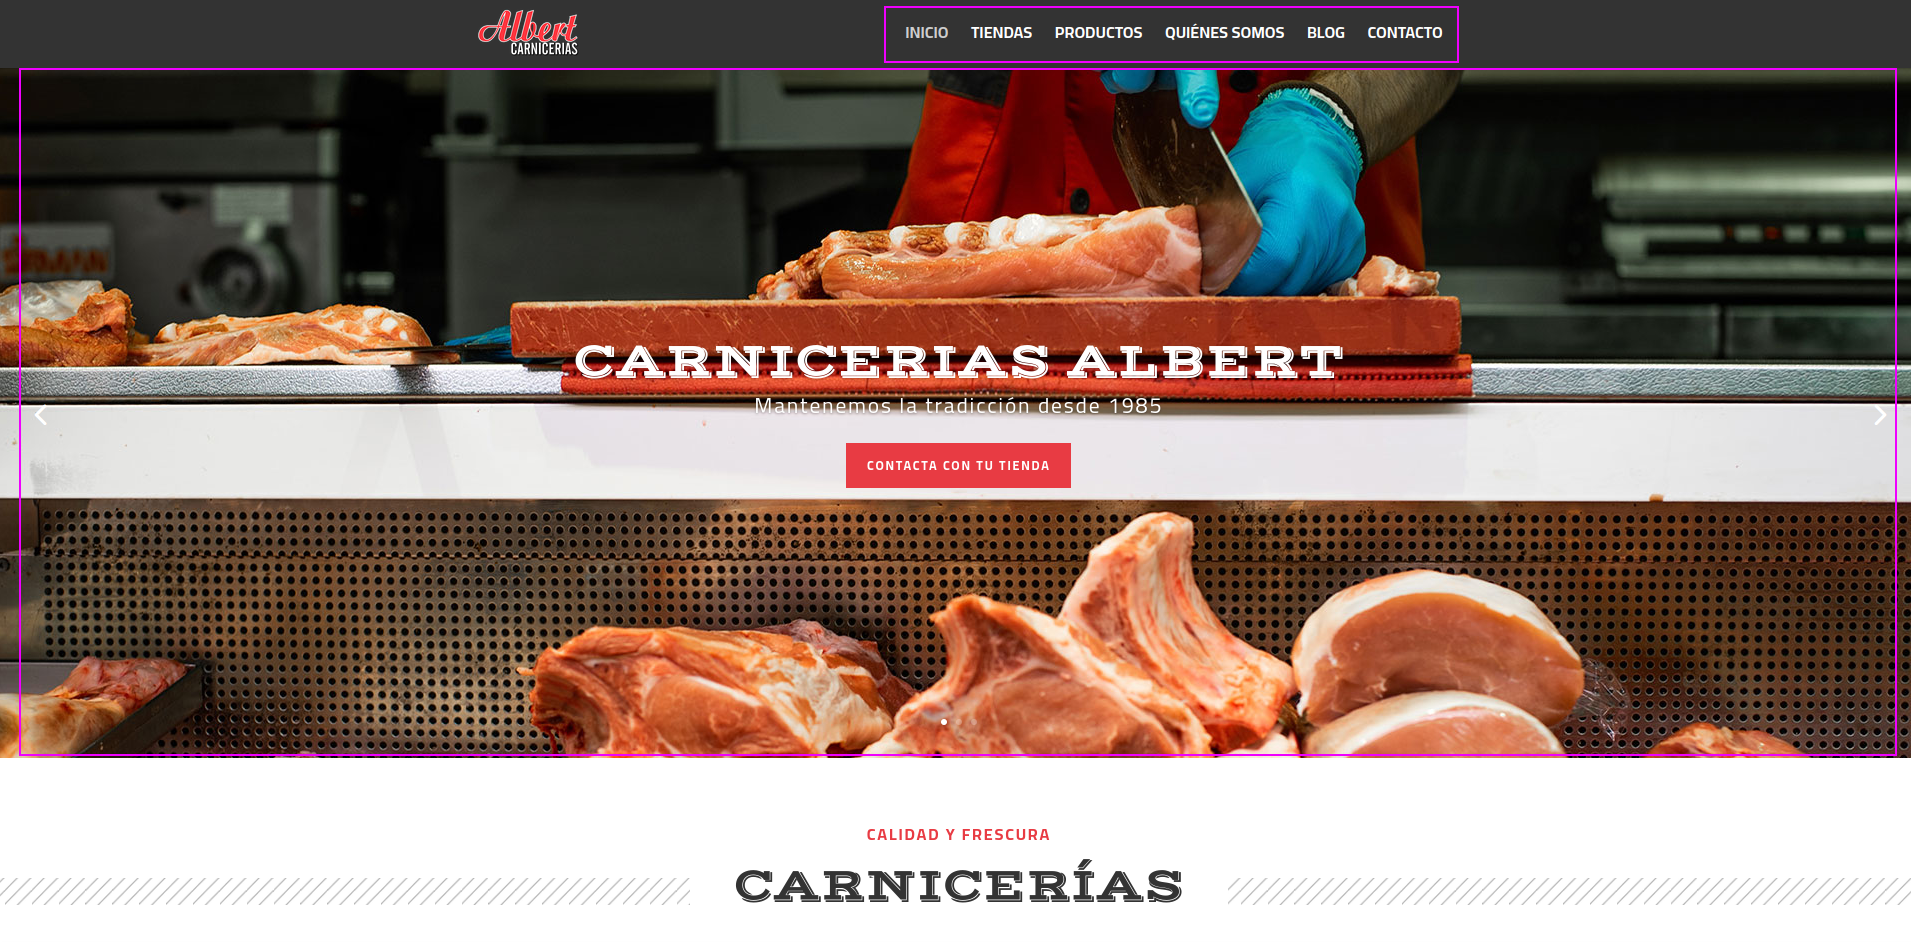
\includegraphics[width=0.75\textwidth]{images/landing-page.png}
\end{figure}

En el \textit{footer} (pie de página) se puede ver un enlace a redes sociales e información de contacto, las cuales están relacionadas con las entradas del menú anteriormente mencionadas.

\begin{figure}[H]
    \centering
    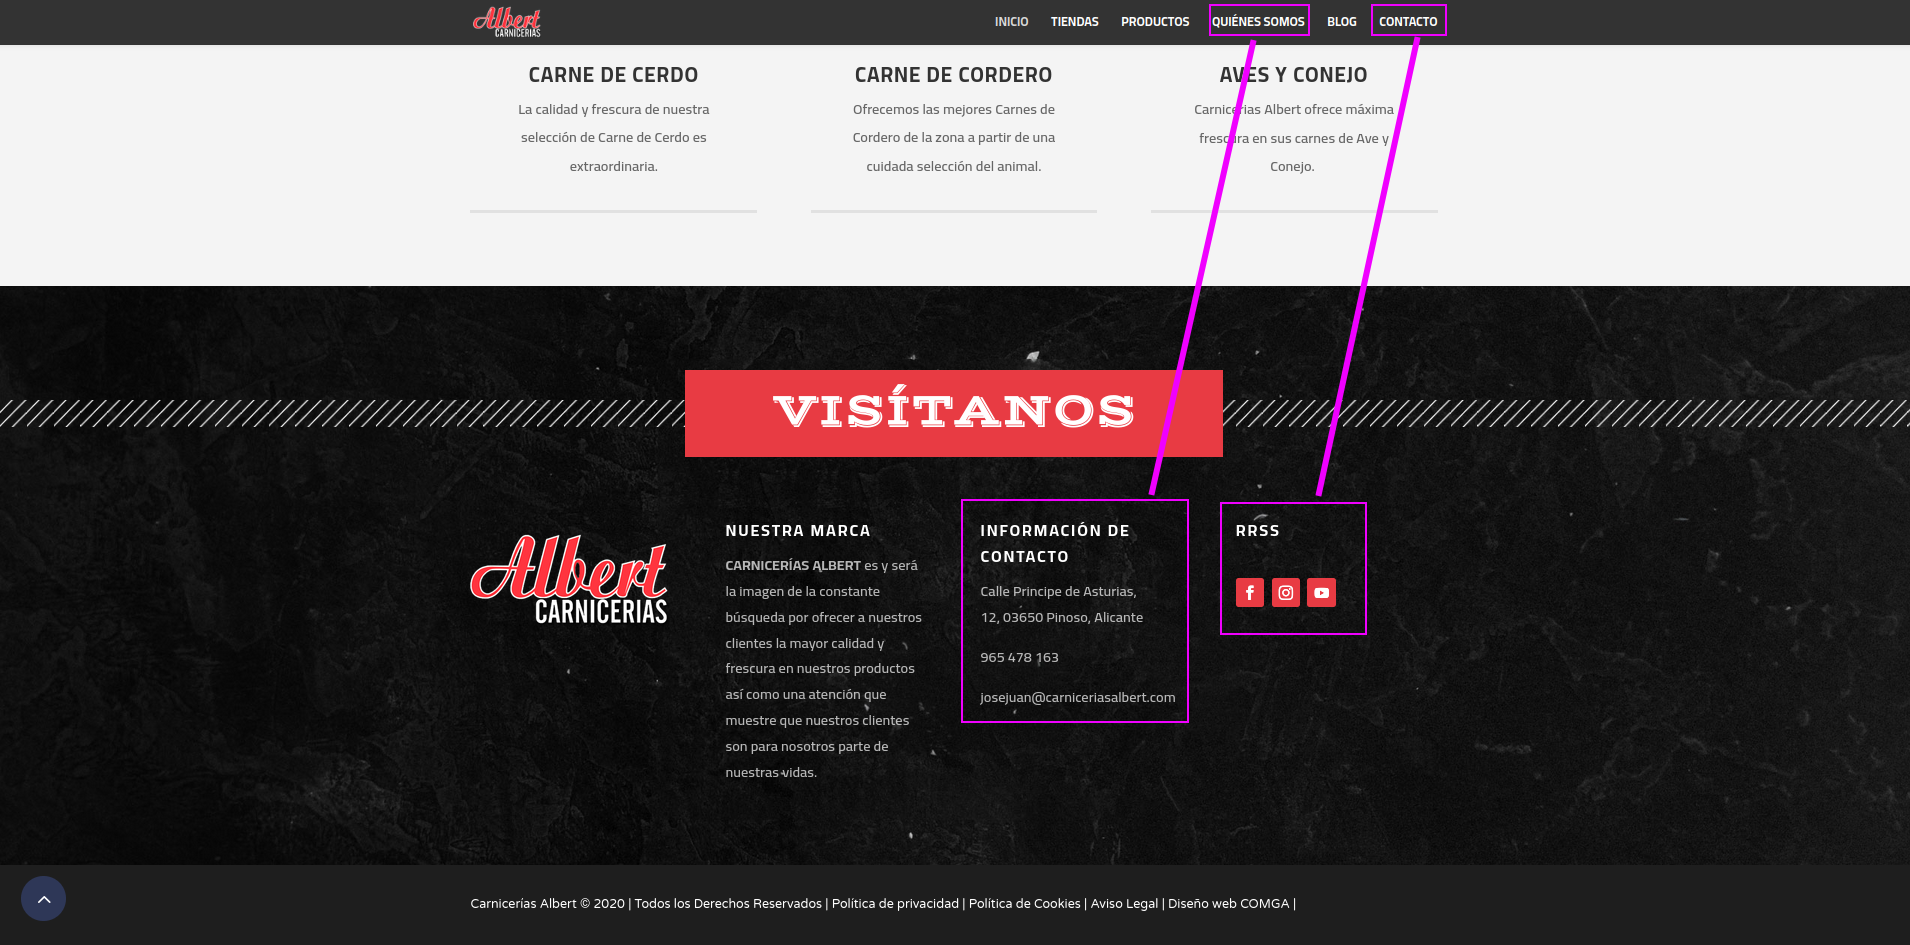
\includegraphics[width=0.75\textwidth]{images/footer.png}
\end{figure}


\subsection{Mockups}

Para visualizar la distribución de los elementos, se han diseñado mockups:

\begin{figure}[H]
    \centering
    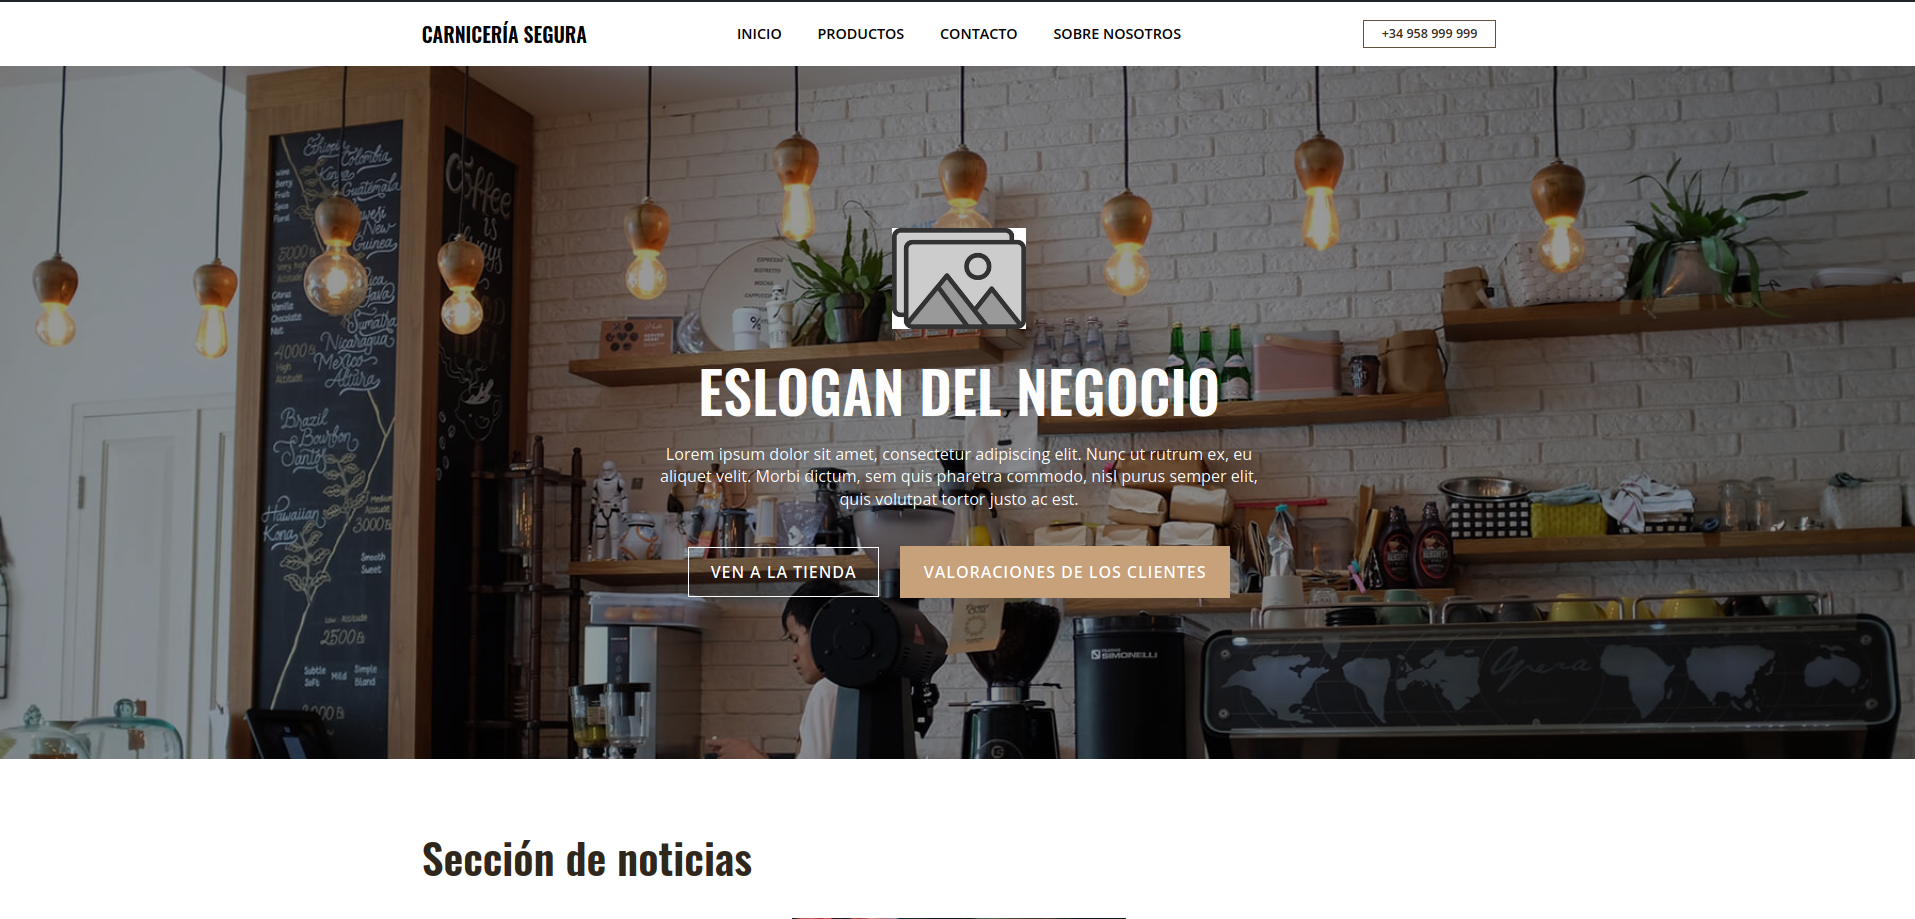
\includegraphics[width=0.75\textwidth]{images/mockup-1.png}
    \captionsetup{width=0.7\textwidth}
    \caption{Cabecera, menú, imágenes y sección de noticias}
\end{figure}

\begin{figure}[H]
    \centering
    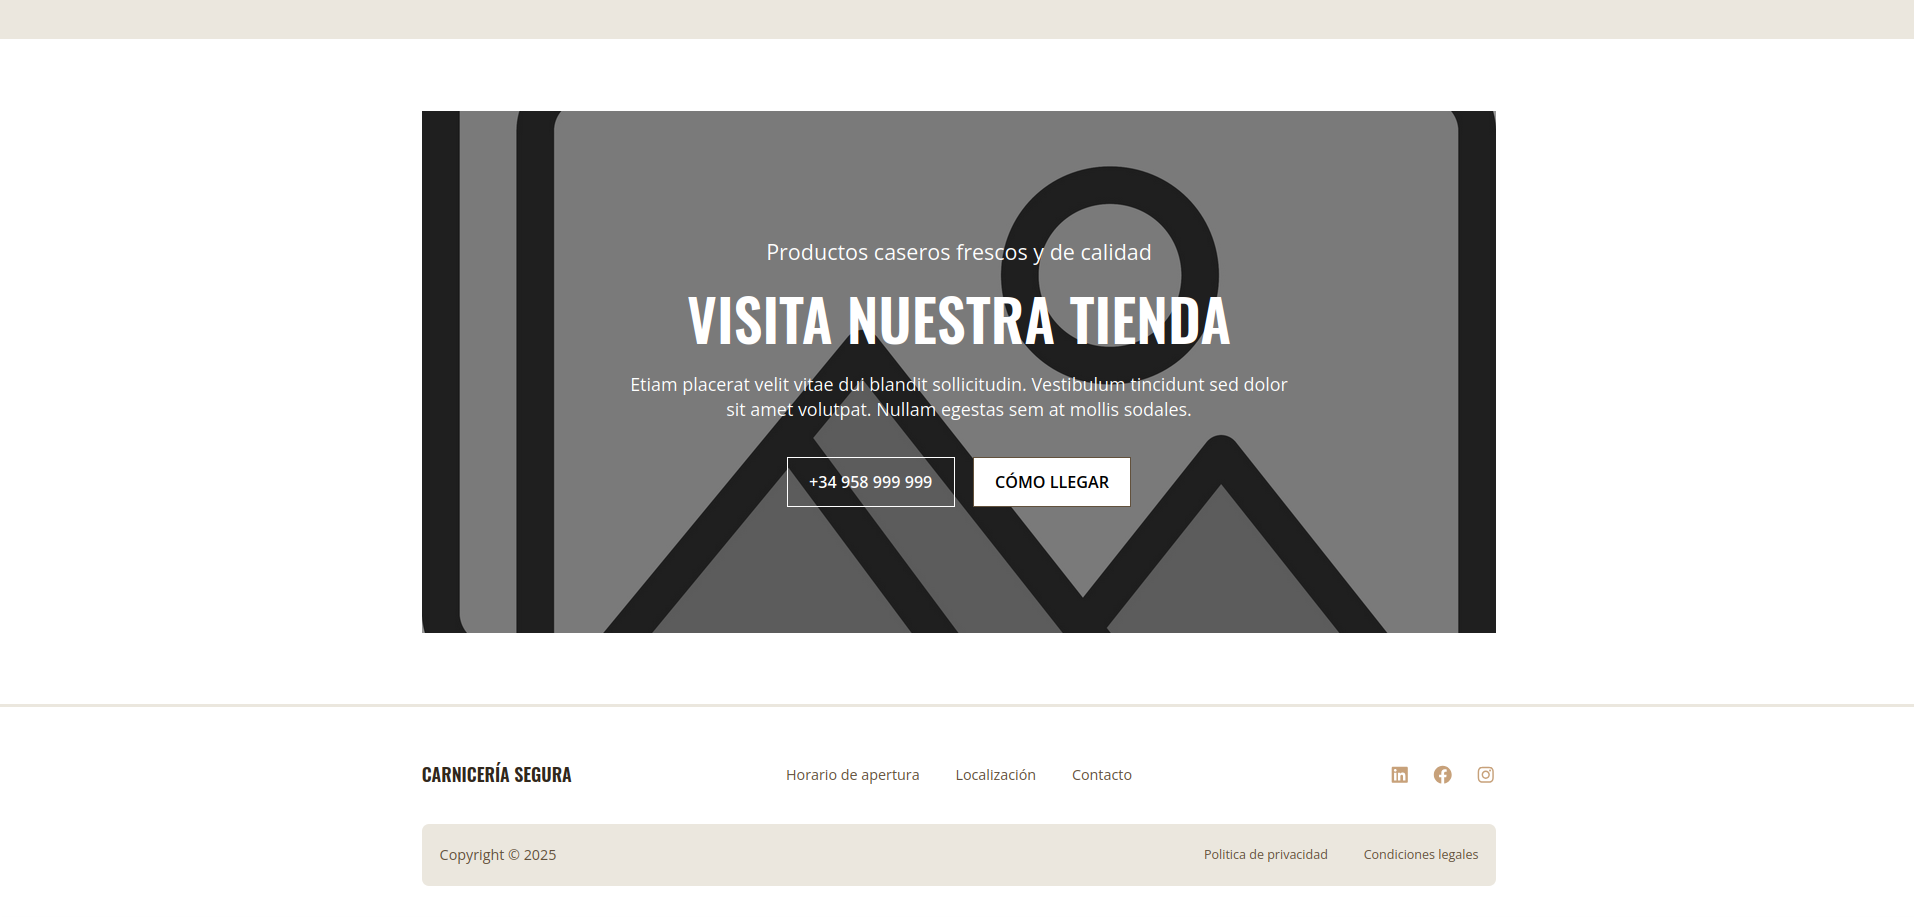
\includegraphics[width=0.75\textwidth]{images/mockup-2.png}
    \captionsetup{width=0.7\textwidth}
    \caption{Pie de página}
\end{figure}

\begin{figure}[H]
    \centering
    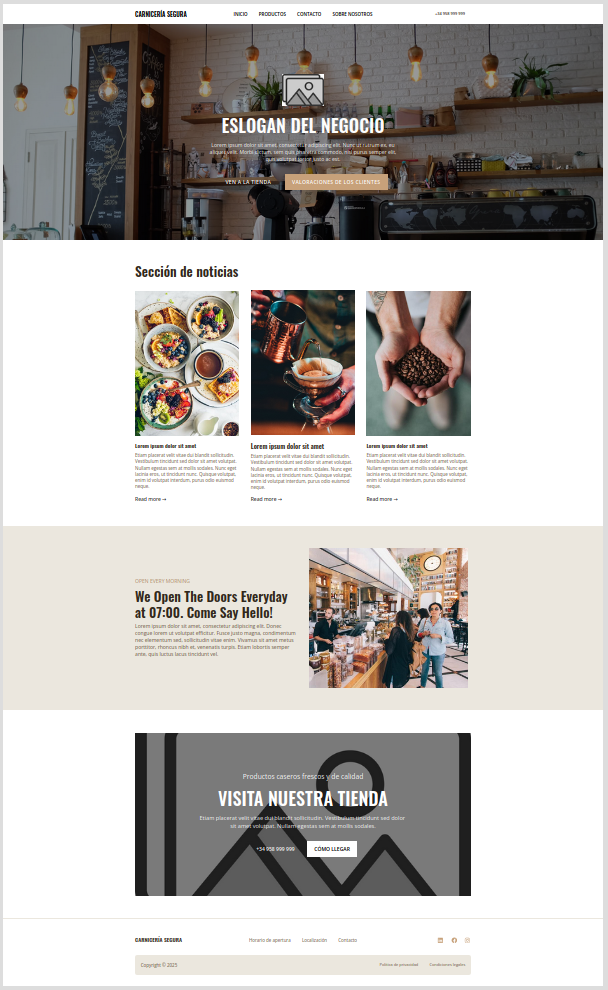
\includegraphics[width=0.9\textwidth]{images/mockup-landing-page.png}
    \captionsetup{width=0.9\textwidth}
    \caption{\textit{Landing page} al completo}
\end{figure}


%%%%%%%%%%%%%%%%%%%%%%%%%%%%%%%%%%%%%%%%%%%%%%%%%%%%%%%%%%%%%%%%%%%%%%%%%%%%%%%%%%%%%%%%%%%%%%%%%%
%%%%%%%%%%%%%%%%%%%%%%%%%%%%%%%%%%%%%%%%%%%%%%%%%%%%%%%%%%%%%%%%%%%%%%%%%%%%%%%%%%%%%%%%%%%%%%%%%%
%%%%%%%%%%%%%%%%%%%%%%%%%%%%%%%%%%%%%%%%%%%%%%%%%%%%%%%%%%%%%%%%%%%%%%%%%%%%%%%%%%%%%%%%%%%%%%%%%%

\section{Planificación del desarrollo}

El desarrollo del CMS se dividirá en las siguientes fases:

\begin{enumerate}

    \item Análisis y Diseño (Semana 1-2): Definir requisitos y funcionalidades. Elaborar mockups.

    \item Desarrollo Inicial (Semana 3-4): Implementar la estructura básica del CMS. Crear sección de noticias y Landing Page.

    \item Galería de productos usando CPT (Semana 5-6): Integrar formulario de pedidos y noticias. Optimizar SEO y seguridad.

    \item Widgets, SEO y seguridad (Semana 7-8): Análisis de Plugins. Creación de widget. Análisis de seguridad y aspectos legales.

\end{enumerate}


\end{document}
